\documentclass{standalone}

\begin{document}

\chapter[Big Data]{Biomedical Big Data - CHIMeRA project}\label{chapter3:bigdata}

\begin{center}
\begin{figure}[htbp]
\centering
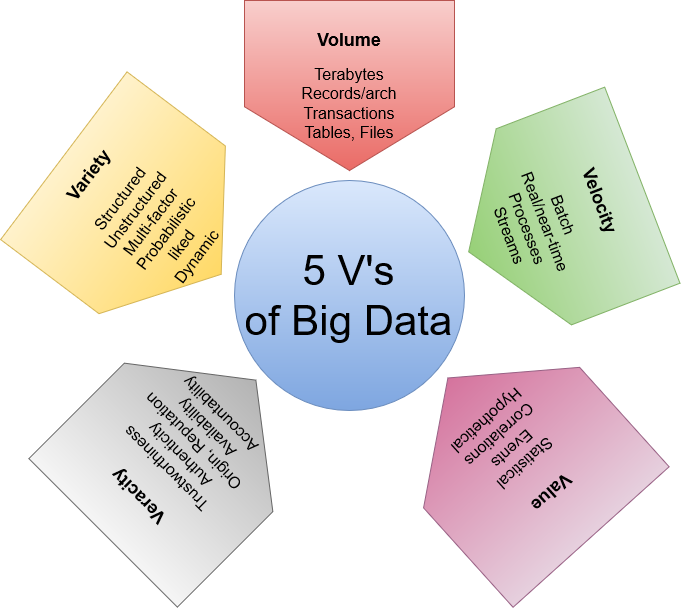
\includegraphics[width=\textwidth]{5v.png}
\caption{Big Data 5 V's}
\label{fig:5v}
\end{figure}
\end{center}

Every second a large quantity of data are produced and shared along the Internet and web-pages.
Data are collected by social networks, chat messages, video streaming and images.
Everyone, in fact, can easily create new data sources and share or put them in Internet pages.
The growth of these data is not limited to multimedia data but it involves many different fields.
This is one of the most important features of the contemporary time, the so-called Big Data era: this huge volume of data is creating a new field in data processing which is called Big Data Analytics, that nowadays is positioned among the top ten strategic technologies (Gartner Research, 2012).

It is still difficult to provide a definition of what exactly are Big Data and we can find many slight different nomenclatures and categories which aim to formulate it.
Moreover, Big Data do not define a particular data type but more than we normally think sources can be labeled as it.
The \emph{International Journal of Computer Applications} defined them as \quotes{$[\cdots]$ a collection of large and complex datasets that cannot be processed and analyzed using traditional computing techniques. It is not a single technique or a tool, rather it involves many areas of business and technology}.
This definition involves many aspects of Big Data processing but it does not provide any definition about their nature.
Moreover, it is easy to identify them as \quotes{big} and thus difficult to analyze, but they are all around us every day and just using the Internet connection every smart-phone or laptop can extract and visualize our web queries.
So could be not properly correct to define them in this way.
However, it is sure that standard computing techniques have to be reviewed to face this vast amount of data and a even more important attention has to be paid on the algorithmic implementations.

While a global definition of Big Data is evidently difficult, we can provide a description of them using some of their \quotes{essential} features.
One of the most common and used set of labels for this purpose is given by the so-called 5 V's of Big Data: volume, velocity, variety, veracity and value.
Despite the first twos are quite obvious (Big Data are certainly \emph{big} in volume and they are produced very \emph{fast}), the remaining three need a particular attention.
We have already treated problems related to the volume of data (ref. Chapter\ref{chapter1:featsel}) and the need of very fast processing and algorithmic optimizations (ref. Chapter\ref{chapter2:neural}), so in this chapter we want to focus on the remaining three characteristics of Big Data Analytics.

As pre-announced, there are many different sources able to provide data and this feature describes the extremely heterogeneity and variety of them.
We can, however, broadly classify this variety into three classes: \emph{structured}, \emph{semi-structured} and \emph{unstructured} data.
A dataset is \emph{structured} if we can easily manage the information in it or, in other words, if it is described using a standard data formats (it is \quotes{quearable}).
On the other side we have the completely \emph{unstructured} datasets, where data are disorganized and we need one or multiple pre-processing steps before handle them.
The intermediate format is given by the \emph{semi-structured} data, in which only a part of them could be handled with standard techniques or we can lead them to their structured version.
The organization of data has been a crucial task in this work of thesis and we will return on this topic in the next sections.

The fourth essential characteristic of Big Data is their \emph{veracity}, due to data inconsistency and incompleteness.
Data are shared very fast using Internet and we can find some ambiguities and/or deceptions between different data sources.
If we want to merge and aggregate different kinds of information (harmonization), we have to face this kind of problems.
The final task of every Big Data Analytic application is, in fact, to process large quantities of data and obtain a unique answer to a problem, which can not vary in relation to the portion of samples or datasets used.

The last, and probably most important feature, is certainly their \emph{value}: it is good to have access to several data but unless we can turn them into valuable information they are useless.
In this vast amount of data only a small part of them can be considered as informative, and it is always hard to extract the informative core.
Moreover, we have to take into account also the difficulties about the management of these data and their more or less complex structure.
However, also in this case, it is hard to generalize this property to all data stored in Internet: every day we see a large quantity of useless information in the Web and it is hard to figure out that some of them can be useful for research applications.
A key role is played by the \emph{questions} which we ask: for every data source, there is always an appropriate question which can be answer using it and which can give a value to it, and vice versa.
In this way also the seemingly useless datasets can acquire importance for an appropriate research project.

In this chapter we are going to discuss about the latest project developed during my PhD, and which is still in work in progress: the \textsf{CHIMeRA} (\emph{Complex Human Interactions in MEdical Records and Atlases}) project.
The project is an extension of a task of the INFN FiloBlu project (ref. next sections and Appendix E for further information about the FiloBlu project) which financed my last PhD year.
\textsf{CHIMeRA} aims to create a unified database of biomedical records, using Natural Language processing techniques.
Its final purpose is to merge multiple data sources available on-line into a single network structure, which highlights the relevant interactions between biomedical information, i.e starting from diseases to the biological agents and compounds involved into their causes and consequences.
The realization of the first version of \textsf{CHIMeRA} has required a lot of time and the development of novel pipelines of data processing.
The project does not still achieve its conclusions, but in this chapter we are going to cross through the main key points which allowed its construction.

%talk about data structured and unstructured
%Many public datasets available.
%Description of the database used in chimera.
%Problems about the intersections and partial information (single db).


\end{document}
